%%%\renewcommand*\printatom[1]{\ensuremath{\mathbf{#1}}}%%lệnh bôi đậm công thức hóa học
\fancyhead[RO,LE]{\color{\mycolor}{\Large\fmmfamily\itshape Chương 1.ESTE - LIPIT}}
\chapter{ESTE-LIPIT}
\section{ESTE}
\subsection{Lý thuyết trọng tâm}
\subsubsection{Khái niệm}
	\begin{kngsnd}
	\begin{minipage}[htp!]{0.6\textwidth}
		Khi ta thay thế nhóm OH trong axit cacboxylic bằng nhóm OH ta thu được este.
		\begin{center}
			\schemestart 
			\chemname{\chemfig{R-C(=[::-90]O)-@{a}{OH}}}{\color{\mycolor!40!black}{Axitcacboxylic}}
			\chemmove{\draw [dashed,red,ultra thick] (a) ellipse ({.4} and {.3});}
			\arrow(.mid east--.mid west){->[\scriptsize{thay nhóm OH}][\scriptsize{bằng nhóm  OR}][0pt]}[0,1.5,,]
			\chemname{\chemfig{R-C(=[::-90]O)-@{b}{OR}}}{\color{\mycolor!40!black}{Este}}
			\chemmove{\draw [dashed,red,ultra thick] (b) ellipse ({.4} and {.3});}
			\schemestop
		\end{center}
		Trong đó: R,R' có thể thuộc loại: no (không chứa liên kết pi) ; không no (chứa liên kết $ \pi $ linh động) hoặc thơm (chứa vòng benzen)
		
		\begin{itemize}
			\item Nếu R và R' đều no: este  no.
			\item Nếu R hoặc R' đều no: este không no.
			\item Nếu R hoặc R' đều no: este thơm.
		\end{itemize}
		Nhóm COO được xem là nhóm chức của este.
	\end{minipage}
\hspace{0pt}
\begin{minipage}[c]{0.4\textwidth}
	Ví dụ: Este: \chemfig{CH_3COOC_2H_5}\\
	Ví dụ:\\
	\setlength{\tabcolsep}{4pt}
	\begin{tabular}{|r|c|}
		\hline
		\chemfig{HCOOCH_3} & \multirow{2}{*}{ este no} \\
		\cline{1-1}
		\chemfig{CH_3COOC_2H_5} &  \\
		\hline
		\chemfig{CH_2=CHCOOCH_3} &  \multirow{3}{*}{ \makecell{este\\ không no} } \\
		\cline{1-1}
		\chemfig{C_2H_5COOCH=CH_2} &  \\
		\cline{1-1}
		\chemfig{CH_2=CHCOOCH=CH_2} &  \\
		\hline	
		\makecell[r]{%
		~	\\
			\chemfig{[:-30]**6(---(-COOCH_3)---)}\\
			       ~
	 } & \multirow{4}{*}{\makecell[c]{este thơm}}  \\
		\cline{1-1}
		\makecell[r]{%
		         ~	\\
			\chemfig{CH_3COO-[:0]**6(------)}\\
		         ~
	}& \\
		\hline	
	\end{tabular}
\end{minipage}
\end{kngsnd}
	\hspace{1cm}
\begin{notegsnd}
		\begin{itemize}
			\item Este đơn chức có một nhóm COO.
			Công thức tổng quát của este no, đơn chức, mạch hở:\chemfig{C_mH_{2m+1}COOC_pH_{2p+1}}\\ ( $ m\geq 0,p \geq 1 $)\\
			Hay \chemfig {C_nH_{2n}O_2}
			\item Este đa chức: có 2 nhóm COO trở lên.
		\end{itemize}
\end{notegsnd}
%
%
%
\vspace{.5cm}
\subsubsection{Danh pháp}
\begin{center}
\tcbox[tcbox width=auto,fontupper=\bfseries\fontfamily{qag}\selectfont,size=small,
on line,before upper=\strut,
colframe=\mycolor!75!black,
colback=\mycolor!5!white]{Tên este RCOOR' = Tên gốc R' + Tên gốc axit RCOO}
\end{center}
	

\begin{hoplythuyet}
\begin{minipage}[htp!]{0.5\textwidth}
	\centering
	{\textbf{Tên một số gốc hiđrocacbon thường gặp}}
	\begin{tabular}{|C{1.2cm}|l|l|l|}
		\hline
		\thead{\sffamily\textbf{\makecell{Phân  \\loại}}}
	 & 
		\multicolumn{2}{c|}{\thead{\sffamily\textbf{Gốc hiđrocacbon}}} & 
		\thead{\sffamily\textbf{Tên gọi}}\\
		\hline
		\multirow{6}{*}{ No} & \multicolumn{2}{l|}{\chemfig{CH_3-}} & metyl\\
		
		& \multicolumn{2}{l|}{\chemfig{C_2H_5-}} & etyl\\
		\cline{2-4}
		& \multirow{2}{*}{ \chemfig{C_3H_7-}} & \chemfig{CH_3CH_2CH_2-}& propyl\\
		
		&  & \chemfig{{(CH_3)}_2CH-} & isopropyl\\
		\cline{2-4}
		& \multicolumn{2}{l|}{\chemfig{CH_3CH_2CH_2CH_2-}} & butyl\\
		
		& \multicolumn{2}{l|}{\chemfig{{(CH_3)}_2CHCH_2CH_2-}} & isoamyl\\
		\hline
		\multirow{2}{*}{\makecell{Không\\ No}}& \multicolumn{2}{l|}{\chemfig{CH_2=CH-}} & vinyl\\
		
		& \multicolumn{2}{l|}{\chemfig{CH_2=CHCH_2-}} & anlyll\\
		\hline
		
		\multirow{4}{*}{Thơm}&\multicolumn{2}{l|}{\makecell[l]{~\\\small\chemfig{[:-30]**6(---(-)---)}\\~\\}} & phenyl\\
		
		& \multicolumn{2}{l|}{\makecell[l]{~\\\small\chemfig{[:-30]**6(---(-CH_2-)----)}\\~\\}} & benzyl\\
		\hline
	\end{tabular}
\end{minipage}
\hspace{-50pt}
\begin{minipage}[htp!]{0.5\textheight}
\centering
{\textbf{Chú ý:Một số este thường gặp}}
\begin{tabular}{|ll|}
	\hline
	\thead{\sffamily\textbf{Công thức cấu tạo}} & \thead{\sffamily\textbf{Tên gọi}} \\
	\hline
	\chemfig{HCOOCH_3} & metyl fomat \\
	\chemfig{HCOOC_2H_5} & etyl fomat \\
	\chemfig{HCOOCH_2CH_2CH_3} & propyl fomat \\
	\chemfig{[,,6,1,,]HCOOCH([:-90,,5,1,,]-CH_3)-CH_3} & isopropyl fomat \\
	\chemfig{CH_3COOCH_3} & metyl axetat \\
	\chemfig{CH_3COOC_2H_5} & etyl axetat \\
	\chemfig{CH_3COOCH_2CH_2CH{(CH_3)}_2} & isoamyl axetat \\
	\chemfig{CH_3COOCH=CH_2} & vinyl axetat \\
	\chemfig{CH_2=CH-COOCH_3} & metyl acrylat \\
	\chemfig{CH_2=CH([:-90,,1,1,,]-CH_3)-COOCH_3} & metyl metacrylat \\
	\makecell[l]{%
		~\\
		\chemfig{CH_3COOCH_2-**6(------)}\\
		~\\
	} & benzyl axetat \\
	\hline
\end{tabular}
\end{minipage}
\hspace{-0.4cm}
\begin{minipage}[htp!]{0.5\textwidth}
\centering
{\textbf{Tên một số gốc axit tương ứng thường gặp}}
\begin{tabular}{|c|l|c|}
	\hline
	\multirow{2}{*}{\thead{\sffamily\textbf{Phân loại}}} & \multicolumn{2}{c|}{\sffamily\textbf{Gốc axit}} \\
	\cline{2-3}
	& \thead{Công thức} & \thead{Tên gọi}\\
	\hline
	\multirow{4}{*}{No}& \chemfig{HCOO-} & fomat\\
	& \chemfig{CH_3COO-} & axetat\\
	& \chemfig{C_2H_5COO-} & propionat\\
	& \chemfig{CH_3CH_2CH_2COO-} & butyrat\\
	\hline
	\multirow{3}{*}{Không No}& \chemfig{CH_2=CHCOO-} & acrylat\\
	& \chemfig{CH_2=C([:-90]-CH_3)([:90]-CH_3)-COO-} & metacrylat\\
	\hline
	Thơm		& \makecell[l]{%
		~\\
		\chemfig{[:-30]**6(---(-COO-)---)}\\
		~\\
	} & benzoat\\
	\hline
\end{tabular}
\end{minipage}

\end{hoplythuyet}


\vspace*{.5cm}
\subsubsection{Tính chất vật lý}

\begin{hoplythuyet}
	\begin{multicols}{2}
		\begin{itemize}
			\item Trạng thái ở đều kiện thường: chất lỏng hoặc rắn
			\item Nhiệt độ nóng chảy và nhiệt độ sôi: Thấp hơn so với ancol và axit cacboxylic có số nguyên tử cacbon và số nhóm chức tương đương.
			\item Tính tan: không tan trong nước, tan nhiều trong dung môi hữu cơ.
			\item Nhiều este có mùi thơm của hoa quả chín
		\end{itemize}
		\columnbreak % chuyển nội dung sang cột khác
		%	\newcolumn Có thể dùng lệnh này để chuyển sang cột khác
		\centering
		{\textbf{Một số este tạo hương vị\\ đặc trưng cho hoa quả}}
		\begin{tabular}{|ll|}
			\hline
			\thead{\sffamily\textbf{Este}} & \thead{\sffamily\textbf{Mùi}} \\
			\hline
			\chemfig{HCOOCH_3} & táo chín \\
			\chemfig{HCOOC_2H_5} & đào chín \\
			\chemfig{CH_3COOC_2H_5} & bơ \\
			\chemfig{CH_3COOCH_2CH_2CH{(CH_3)}_2} & chuối chín \\
			\hline
			\chemfig{C_2H_5COOC_2H_5} & \multirow{2}{*}{dứa} \\
			\chemfig{C_3H_7COOC_2H_5} &  \\
			\hline
			\makecell[l]{%
				~\\
				\chemfig{CH_3COOCH_2-**6(------)}\\
			     ~\\
		} & hoa nhài \\
			\hline
		\end{tabular}
	\end{multicols}
\end{hoplythuyet}

\subsubsection{Tính chất hóa học}
\paragraph{Phản ứng thủy phân trong môi trường axit}
\begin{center}
\schemestart
 \chemfig{RCOOR'}
 \+
 \chemfig{H_2O}
 \arrow{<=>[$\scriptsize t^\circ $][$H_2{SO_4}_\text{đặc} $]}[,1.5,,]
 \chemfig{RCOOH}
 \+
 \chemfig{R'OH}
 \schemestop
\end{center}
 \begin{itemize}
 \item \textbf{Đặc điểm:} phản ứng thuận nghịch
 \end{itemize}
\paragraph{Phản ứng thủy phân trong môi trường bazơ}

\begin{center}
\schemestart
\chemfig{RCOOR'}
\+
\chemfig{NaOH}
\arrow{->[$\scriptsize t^\circ $][]}[,1.5,,]
\chemfig{RCOONa}
\+
\chemfig{R'OH}
\schemestop
\end{center}
\begin{itemize}
	\item \textbf{Đặc điểm:} phản ứng một chiều
	\item \textbf{Tên gọi:} Phản ứng xà phòng hóa
\end{itemize}

\paragraph{Phản ứng cộng và phản ứng trùng hợp của este không no}

\begin{hoplythuyet}

\begin{minipage}[t]{.3\textwidth}
	\begin{itemize}
	\item Các este không no có thể tham gia phản ứng cộng \chemfig{H_{2}}(xúc tác, $ t^\circ $), cộng \chemfig{Br_{2}}, cộng HX(X là gốc axit) và phản ứng trùng hợp.
	\item Một số este đơn giản có liên kết C=C tham gia phản ứng trùng hợp giống như anken.
	\end{itemize}
\end{minipage}
\hspace*{10pt}
\begin{minipage}[t]{.7\textwidth}
\textbf{Ví dụ 1:}\\
\schemestart 
\chemfig{CH_{2}=CHCOOCH_{3}}
\+
\chemfig{H_{2}}
\arrow{->[$ t^\circ $][Ni][]}[,1,,]
\chemfig{CH_{3}CH_{2}COOCH_{3}}
\schemestop

\textbf{Ví dụ 2:}\\
\schemestart 
\chemfig{CH_{2}=CHCOOCH_{3}}
\+
\chemfig{Br_{2}}
\arrow{->[$ t^\circ $][Ni][]}[,1,,]
\chemfig{CH_{2}BrCHBrCOOCH_{3}}
\schemestop

\textbf{Ví dụ 3:}\\
\schemestart 
\chemname{\chemfig{nCH_{2}=CH-C(=[:-90]O)-O-CH_{3}}}{metyl acrylat}
\arrow(.mid east--.mid west){->[\scriptsize{xt, $ t^\circ$}][][]}[,1,,]
\chemname{%
	\chemfig{%
		\vphantom{CH_2}-[@{lef,.75}]CH(-[:-90]COOCH_{3})-CH_{2}-[@{rig,.25}]
	}
	\polymerdelim[%
	height = 6pt,
	indice = \!\!n,
	depth = 15pt,
	%delimiters ={[]},
	%open xshift = -10pt
	]{lef}{rig}
}
{poli(metyl acrylat)}
\schemestop
\end{minipage}

\end{hoplythuyet}

\paragraph{Phản ứng cháy}

\begin{hoplythuyet}
\begin{minipage}[t]{.3\textwidth}
Các este dễ cháy và tỏa nhiều nhiệt:
\end{minipage}
\hspace{10pt}
\begin{minipage}[t]{.7\textwidth}
	\textbf{Ví dụ 4:}\\
	\schemestart 
	\chemfig{CH_{3}COOC_{2}H_{5}}
	\+
	\chemfig{5O_{2}}
	\arrow{->[$ t^\circ $][][]}[,1,,]
	\chemfig{4CO_{2}}
	\+
	\chemfig{4H_{2}O}
	\schemestop
\end{minipage}
\end{hoplythuyet}

\begin{notegsnd}
	R'OH sinh ra có thể phản ứng với môi trường (nếu là phenol) hoặc không bền chuyền hóa thành anđehit, xeton.
	\begin{itemize}
		\item Este $+\mathrm{NaOH} \rightarrow$ Muối + anđehit:\par
      \schemestart
      \chemfig{RCOOCH=CHR'}
      \+
      \chemfig{NaOH}
       \arrow{->[$ t^\circ $][][]}[0,.7,,]
       \chemfig{RCOONa}
       \+
       \chemfig{R'CH_2CHO}
       \schemestop
		
		\item Este $+\mathrm{NaOH} \rightarrow$ Muối + xeton:\par
		 \schemestart
		\chemfig{RCOOC(-[:-90,,5,1,,]R'')=CHR'}
		\+
		\chemfig{NaOH}
		\arrow(.mid east--.mid west){->[$ t^\circ $][][]}[0,.7,,]
		\chemfig{RCOONa}
		\+
		\chemfig{R'CH_2C(=[:-90,,4,1,,]O)-R''}
		\schemestop
		\item Este $+\mathrm{NaOH} \rightarrow 2 \mathrm{\text{Muối}}+\mathrm{H}_2 \mathrm{O}$:\par
		
		 \schemestart
		\chemfig{RCOO-**6(---(-R')---)}
		\+
		\chemfig{2NaOH}
		\arrow{->[$ t^\circ $][][]}[0,.7,,]
		\chemfig{RCOONa}
		\+
		\chemfig{R'-**6(---(-ONa)---)}
		\+
		\chemfig{H_2O}
		\schemestop
		
	\end{itemize}
\end{notegsnd}
\newpage
\subsubsection{Điều chế và ứng dụng}
\paragraph{Điều chế}

\begin{hoplythuyet}
	{\sffamily\textbf{Este của ancol}}\\
	
	\begin{itemize}
		\item \textbf{Phương pháp:} Đun hồi lưu ancol với axit hữu cơ
		\item Dùng \chemfig{H_{2}SO_{4}} vừa làm chất xúc tác vừa làm chất hút nước để tăng hiệu suất phản ứng.
	\end{itemize}
	
\begin{center}
	\schemestart 
\chemfig{CH_{3}COOH}
\+
\chemname{\chemfig{{(CH_{3})}_{2}CHCH_{2}CH_{2}OH}}{ancol isoamylic}
\arrow(.mid east--.mid west){<=>[\scriptsize$ t^\circ $][\scriptsize\chemfig{H_2SO_4}][]}[,1,,]
\chemname{\chemfig{CH_{3}COOCH_2CH_2CH{(CH_3)}_2}}{isoamyl axetat}
\+
\chemfig{H_2O}
\schemestop
\end{center}
	
	{\sffamily\textbf{Este của phenol}}:
	
	\begin{itemize}
		\item \textbf{Phương pháp:} Dùng anhidrit axit tác dụng với phenol và phản ứng xảy ra một chiều.
		\item \textbf{Chú ý:}: không dùng phenol tác dụng với axit cacboxylic
	\end{itemize}
	
	\begin{center}
		\schemestart 
		\chemfig{[:-30]**6(---(-OH)---)}
		\+
		\chemname{\chemfig{CH_3-C(=[:-90]O)-O-C(=[:-90]O)-CH_3}}{anhiđrit axit}
		\arrow(.mid east--.mid west){->[][][]}[,1,,]
		\chemname{\chemfig{CH_{3}COO-**6(------)}}{phenyl axetat}
		\+
		\chemfig{CH_{3}COOH}
		\schemestop
	\end{center}
	
\end{hoplythuyet}

\paragraph{Ứng dụng}
\begin{hoplythuyet}
	\begin{itemize}
	\item 	Công nghiệp hương liệu và mùi hương 
	\item 	Ngành thực phẩm , đồ uống và mỹ phẩm
	\item   Công nghiệp sơn và mực in
	\item   Dược phẩm
	\end{itemize}
\end{hoplythuyet}
\newpage
\begin{tikzpicture}[overlay,remember picture,declare function={d=5cm;}]
	\path 
	(0,0) coordinate (O)
	(d,0) coordinate (A)
	($ (O)!1!90:(A) $) coordinate (B)
	($ (O)!1!180:(A) $) coordinate (C)
	($ (O)!1!270:(A) $) coordinate (D)
	;
	\begin{scope}[transform canvas={xshift=8.5cm,yshift=-8cm}]
		
		\begin{scope}%[transform canvas={xshift=3cm,yshift=-3cm}]
			\clip (A) coordinate (E)  circle (2.3);
			\path (E) node(Et){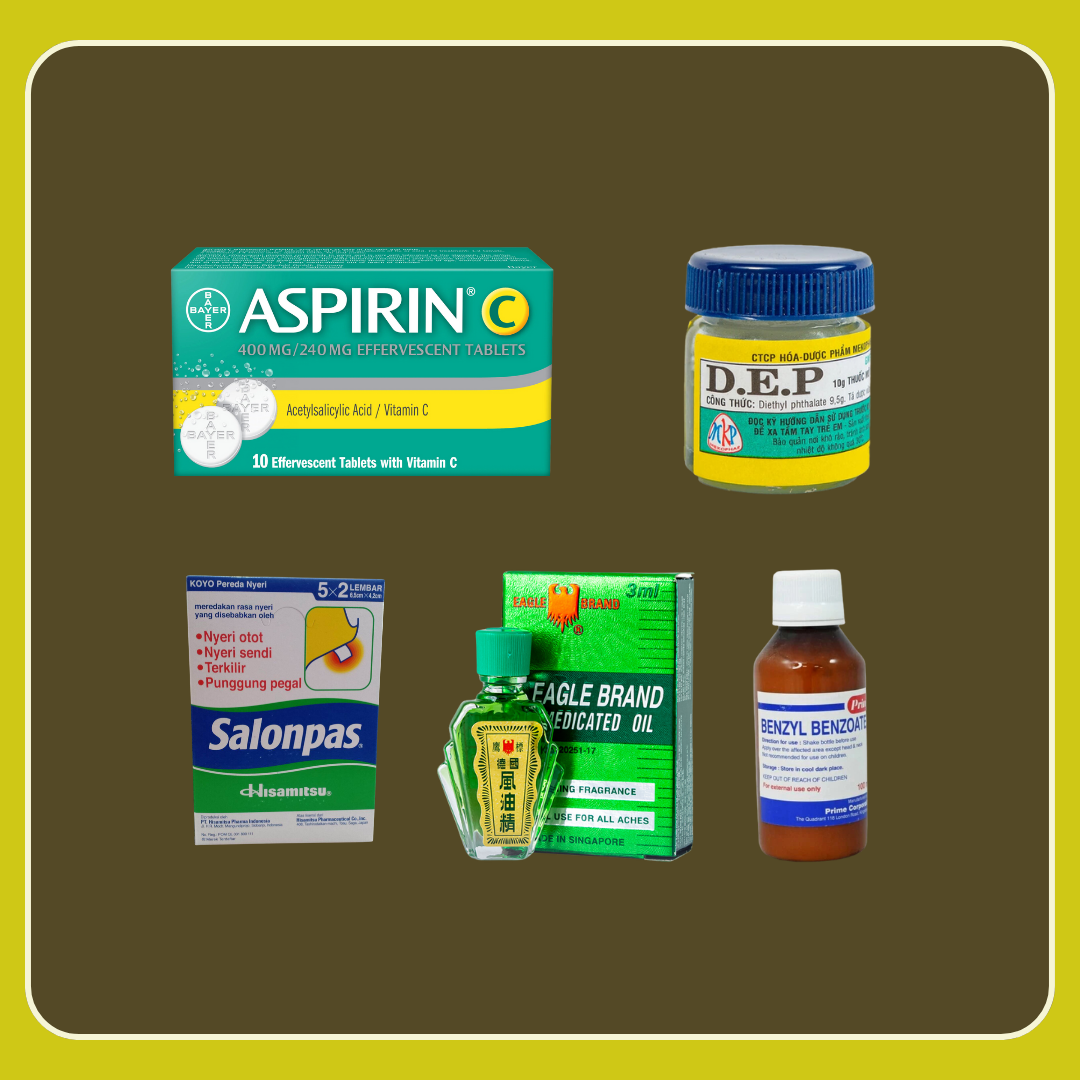
\includegraphics[width=5cm]{duocpham.png}};
			\draw[\mycolor,line width=3pt] (E) circle (2.3);
			
		\end{scope}
		\path (Et.south) node[anchor=north,\mycolor!50!black,font=\fontsize{14pt}{6pt}\bfseries\sffamily]{Dược phẩm}
		;
		
		\begin{scope}%[transform canvas={xshift=3cm,yshift=-3cm}]
			\clip (B) coordinate (F)  circle (2.3);
			\path (F) 
			node (Ft) {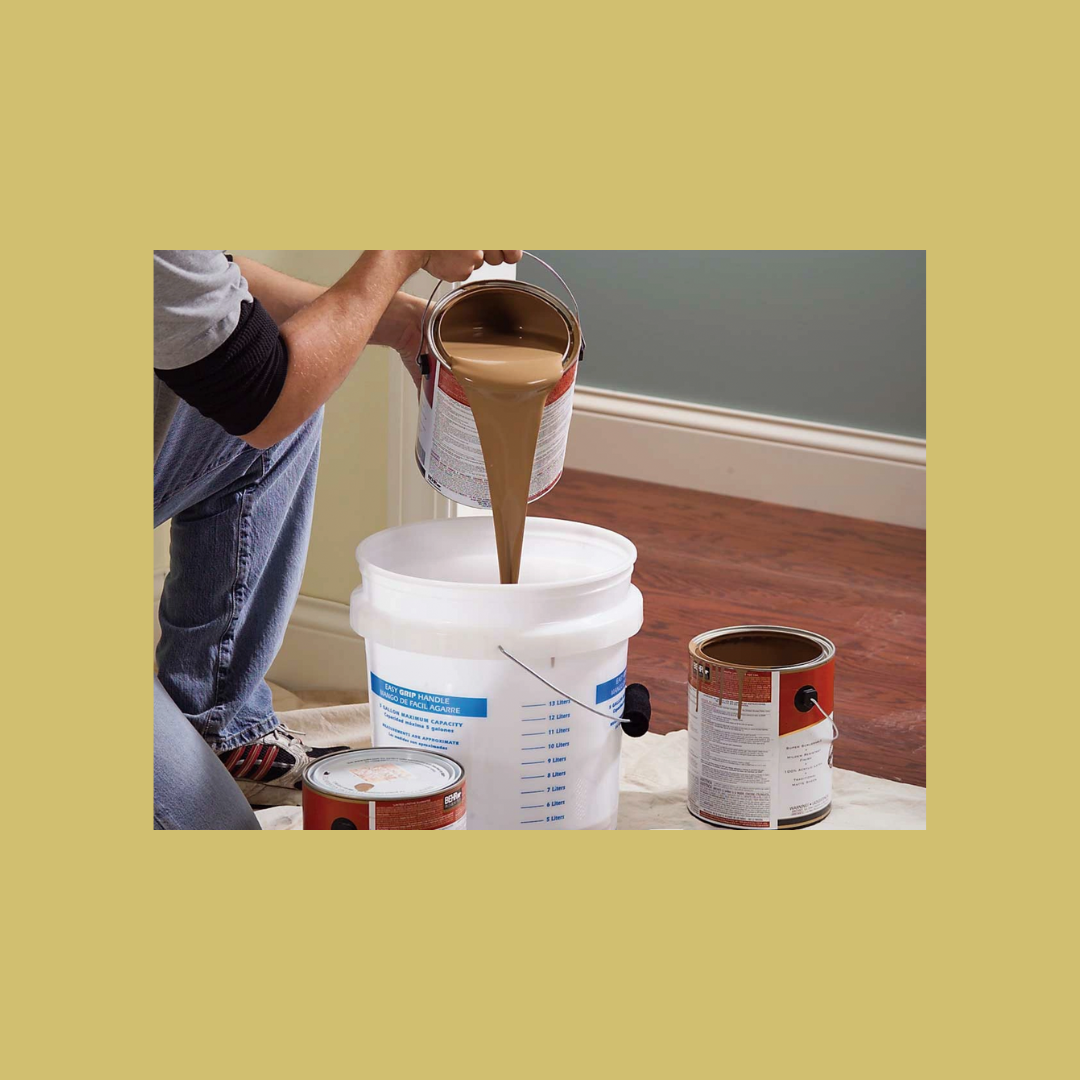
\includegraphics[width=5cm]{son.png}}
			;
			\draw[\mycolor,line width=3pt] (F) circle (2.3);
			
		\end{scope}
	\path (Ft.east) node[anchor=west,\mycolor!50!black,font=\fontsize{14pt}{6pt}\bfseries\sffamily]{Pha sơn,\\ mực in}
	;
	
	
		
		\begin{scope}%[transform canvas={xshift=3cm,yshift=-3cm}]
			\clip (C) coordinate (G)  circle (2.3);
			\path (G) node(Gt){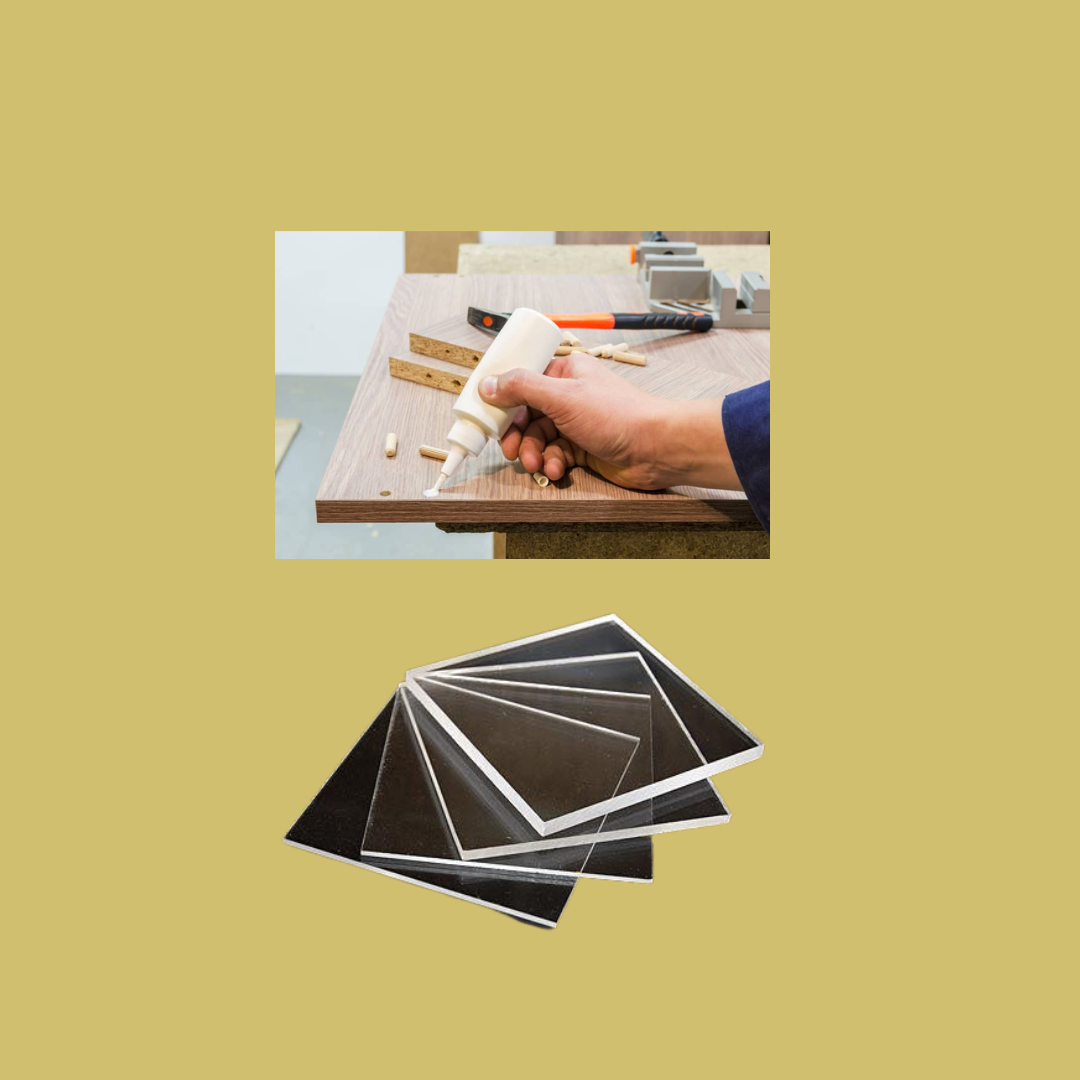
\includegraphics[width=5cm]{chatdeo.png}};
			\draw[\mycolor,line width=3pt] (G) circle (2.3);
		\end{scope}
			\path (Gt.north) node[anchor=south,\mycolor!50!black,font=\fontsize{14pt}{6pt}\bfseries\sffamily]{Chất dẻo,\\
				thủy tinh hữu cơ}
		;
		
		\begin{scope}%[transform canvas={xshift=3cm,yshift=-3cm}]
			\clip (D) coordinate (H)  circle (2.3);
			\path (H) node(Ht){
\includegraphics[width=5cm]{mypham.png}};
			\draw[\mycolor,line width=3pt] (H) circle (2.3);
		\end{scope}
	
		\path (Ht.west) node[anchor=east,\mycolor!50!black,font=\fontsize{14pt}{6pt}\bfseries\sffamily]{Hương liệu,\\
	mỹ phẩm}
	;
	\end{scope}
\end{tikzpicture}

\newpage
\subsection{Bài tập tự luận}

\Opensolutionfile{ansbt}[Ans/BTESTE]
%%%%%%%%%%%%%%%%%%%%%%%%============Bắt đầu Bài tập 1=================%%%%%%%%%%%%%%%%
\begin{bt}[2 điểm][Đồng phân este]
	Viết đồng phân của các hợp chất đơn chức (axit và este) có công thức sau: \chemfig{C_2H_4O_2},\chemfig{C_3H_6O_2},\chemfig{C_4H_8O_2},\chemfig{C_4H_6O_2}.
	\sodongkebt[\cauTH]
	\loigiai
	{%
		Nội dung lời giải bài 1}
\end{bt}
%%%%%%%%%%%%%%%%%%%%%%%%============Kết thức Bài tập 1=================%%%%%%%%%%%%%%%%
%%%%%%%%%%%%%%%%%%%%%%%%============Bắt đầu Bài tập 2=================%%%%%%%%%%%%%%%%
\begin{bt}[2 điểm][Danh pháp este]
	Gọi tên hoặc viết công thức của các este trong bảng sau:
	
\vspace{12pt}
\begin{tabular}{|l|l|l|l|}
	\hline
\rowcolor{\mauphu!20}
{\sffamily\textbf{Công thức}} & {\sffamily\textbf{Tên gọi}}  & {\sffamily\textbf{Tên gọi}} & {\sffamily\textbf{Công thức}} \\
\hline
(1) \chemfig{HCOOCH_3}&  & (7) metyl axetat & \\

(2) \chemfig{CH_3COOCH=CH_2}&  & (8) isoamyl axetat & \\

(3) \makecell
{%
	~\\
	\chemfig{[:-30]**6(---(-COO-**6(------))---)}\\
	~\\
}
&  & (9) metyl metacrylat & \\

(4) \chemfig{C_2H_5COOCH_2CH=CH_2}&  & (10) isopropyl propionat & \\
(5) \makecell{
~\\
	\chemfig{HCOO-**6(------)}\\
~\\
}&  & (11) etyl fomat & \\

(6)   \chemfig{CH_3OOC-COOCH_3}    &   & (12)  metyl acrylat    &\\


\hline
\end{tabular}

\vspace{12pt}

Hãy cho biết trong các este trên những este nào:
\begin{enumerate}
	\item thủy phân tạo thành ancol: \dotfill
	\item thủy phân thu được sản phẩm có khả năng tráng gương:  \dotfill
    \item làm mất màu dung dịch brom: \dotfill
    \item có khả năng tham gia phản ứng trùng hợp \dotfill
\end{enumerate}
	\sodongkebt[6]
	\loigiai
	{%
		Nội dung lời giải bài 1}
\end{bt}
%%%%%%%%%%%%%%%%%%%%%%%%============Kết thức Bài tập 2=================%%%%%%%%%%%%%%%%
%%%%%%%%%%%%%%%%%%%%%%%%============Bắt đầu Bài tập 3=================%%%%%%%%%%%%%%%%


\begin{bt}[2][Viết phương trình phản ứng]
	\begin{enumerate}
	\item So sánh phản ứng thủy phân trong ding dịch axit và trong dung dịch kiềm.
	\item Hoàn thành các phương trình phản ứng sau:
	\begin{enumerate}
		\item \schemestart 
		\chemfig{CH_3COOCH_2CH_2CH{(CH_3)}_2}
		\+
		\chemfig{H_2O}
		\arrow{->[\scriptsize$ H^+,t^\circ $][][]}[,1,,]
		\phantom{\chemfig{CH_3COOCH_2CH_2CH{(CH_3)}_2} }
		\schemestop
		
		
		\item \schemestart 
		\chemfig{CH_3COOCH_2CH_2CH{(CH_3)}_2}
		\+
		\chemfig{H_2O}
		\arrow{->[\scriptsize$ H^+,t^\circ $][][]}[,1,,]
		\phantom{\chemfig{CH_3OOCCH_2CH_2CH{(CH_3)}_2} }
		\schemestop
		
		
		\item \schemestart 
		\chemfig{[:-30]**6(---(-OOCCH_3)---)}
		\+
		\chemfig{NaOH}
		\arrow{->[\scriptsize\chemfig{H_2O},$t^\circ $][][]}[,1,,]
		\phantom{\chemfig{CH_3OOCCH_2CH_2CH{(CH_3)}_2} }
		\schemestop
		
		
		\item \schemestart 
		\chemfig{[:-30]**6(---(-COOCH_3)---)}
		\+
		\chemfig{NaOH}
		\arrow{->[\scriptsize\chemfig{H_2O},$t^\circ $][][]}[,1,,]
		\phantom{\chemfig{CH_3OOCCH_2CH_2CH{(CH_3)}_2} }
		\schemestop
		
	\end{enumerate}
	\end{enumerate}
	\sodongkebt[\cauTH]
\end{bt}

%%%%%%%%%%%%%%%%%%%%%%%%============Kết thức Bài tập 3=================%%%%%%%%%%%%%%%%
%%%%%%%%%%%%%%%%%%%%%%%%============Bắt đầu Bài tập 4=================%%%%%%%%%%%%%%%%
\begin{bt}[2][chuỗi phản ứng]
	Hoàn thành chuỗi phản ứng sau:\\ 
\schemestart
\chemfig{CH_3COONa}
\arrow(a1--a2){->[\scriptsize$ (1) $][][]}[,.6,,,]
\chemfig{CH_4}
\arrow(--a3){->[\scriptsize$ (2) $][][]}[,.6,,,]
\chemfig{C_2H_2}
\arrow(--a4){->[\scriptsize$ (3) $][][]}[,.6,,,]
\chemfig{C_2H_4}
\arrow(--a5){<=>[\scriptsize$ (4) $][\scriptsize$ (5) $][]}[,.6,,,]
\chemfig{C_2H_5OH}
\arrow(--a6){->[\scriptsize$ (6) $][][]}[,.6,,,]
\chemfig{CH_3COOH}
\arrow(--a7){<=>[*{0}\scriptsize$ (7) $][*{0}\scriptsize$ (8) $][]}[-90,.6,,,]
\chemfig{CH_3COOC_2H_5}
	\arrow(--a8){->[\scriptsize$ (9) $][][]}[180,.6,,,]
	\chemfig{CH_3COONa}
\schemestop
\sodongkebt[\cauTH]
\end{bt}

%%%%%%%%%%%%%%%%%%%%%%%%============Kết thức Bài tập 4=================%%%%%%%%%%%%%%%%
%%%%%%%%%%%%%%%%%%%%%%%%============Bắt đầu Bài tập 5=================%%%%%%%%%%%%%%%%


\begin{bt}[2][Phát biểu đúng sai về este]
Các phát biểu sau đúng hay sai? Hãy giải thích.

\begin{enumerate}[(1)]
	\item Este no, đơn chức, mạch hở có công thức phân tử \chemfig{C_nH_{2n}O_2}, với $ n \geq 2 $.
	
	\dotfill
	\item Các este là những chất lỏng, nhẹ hơn nước, rất ít tan trong nước, có khả năng hòa tan nhiều chất hữu cơ khác nhau.
	
	\dotfill
	\item Este vinyl axetat có đồng phân hình học.
	
	\dotfill
	
	\item \chemfig{HCOOCH_3} có nhiệt độ sôi cao hơn \chemfig{C_2H_5OH} do có phân tử khối lớn hơn.
	
	\dotfill
	
	\item Có 2 este đơn chức X đều có tỉ khối hơi so với \chemfig{H_2} bằng $ 30 $. 
	
	\dotfill
	
	\item Thủy phân vinyl axetat trong môi trường kiềm thu được muối và anđehit.
	
	\dotfill
	
	\item Phản ứng thủy phân este trong môi trường kiềm là phản ứng một chiều.
	
	\dotfill
	
   \item Phản ứng thủy phân este trong môi trường axit gọi là phản ứng xà phòng hóa
   
   \dotfill
	
	 \item Các este đều được điều chế từ axit cacboxylic và ancol. 
	
	\dotfill
	
	
\end{enumerate}
\sodongkebt[\cauTH]
\end{bt}

%%%%%%%%%%%%%%%%%%%%%%%%============Kết thức Bài tập 5=================%%%%%%%%%%%%%%%%
%%%%%%%%%%%%%%%%%%%%%%%%============Bắt đầu Bài tập 6=================%%%%%%%%%%%%%%%%


\begin{bt}[3]
	Hoàn thành các phương trình phản ứng sau (ghi rõ điều kiện nếu có):
	\setchemfig{arrow style={dashed,>=stealth,line width =.9pt}}
	\begin{enumerate}
		\item \schemestart
		\chemfig{HCOOC_2H_5}
		\+
		\chemfig{NaOH}
		\arrow{->[][][]}[,.7,,]
        \ldots\ldots\ldots\ldots
        \+
        \ldots\ldots\ldots\ldots
		 \schemestop
		 
		 \item \schemestart
		 \chemfig{CH_3OCOC_2H_5}
		 \+
		 \chemfig{H_2O}
		 \arrow{->[][][]}[,.7,,]
		 \ldots\ldots\ldots\ldots
		 \+
		 \ldots\ldots\ldots\ldots
		 \schemestop
		 
		 \item \schemestart
		 \chemfig{CH_3COOCH=CH_2}
		 \+
		 \chemfig{NaOH}
		 \arrow{->[][][]}[,.7,,]
		 \ldots\ldots\ldots\ldots
		 \+
		 \ldots\ldots\ldots\ldots
		 \schemestop
		 
		 \item \schemestart
		 \chemfig{CH_2=C(-[:-90,1,1]CH_3)-COOCH_3}
		 \+
		 \chemfig{NaOH}
		 \arrow(.mid east--.mid west){->[][][]}[,.7,,]
		 \ldots\ldots\ldots\ldots
		 \+
		 \ldots\ldots\ldots\ldots
		 \schemestop
		 
		 
		 
		  \item \schemestart
		 \chemfig{CH_3COO-*6(=-=-=-)}
		 \+
		 \chemfig{NaOH}
		 \arrow(.mid east--.mid west){->[][][]}[,.7,,]
		 \ldots\ldots\ldots\ldots
		 \+
		 \ldots\ldots\ldots\ldots
		 \schemestop
		 
		 
		  \item \schemestart
		 \chemfig{*6(=-(-[:-30]OH)=(-[:30]COOH)-=-)}
		 \+
		 \chemfig{CH_3OH}
		 \arrow(.mid east--.mid west){->[][][]}[,.7,,]
		 \ldots\ldots\ldots\ldots
		 \+
		 \ldots\ldots\ldots\ldots
		 \schemestop
		 
	\end{enumerate}
\sodongkebt[6]
\end{bt}
\Closesolutionfile{ansbt}
%
%
%
%%%%%%%%%%%%%%%%%%%%%%%%============Kết thức Bài tập 6=================%%%%%%%%%%%%%%%%
%%%%%%%%%%%%%%%%%%%%%%%%============Bắt đầu ví dụ 1=================%%%%%%%%%%%%%%%%
%
%
%
\subsection{Bài tập trắc nghiệm}

\begin{dangntd}{Lí thuyết trọng tâm}
	\begin{ntdppg}{Phương pháp giải}
		Cần nắm vững lý thuyết khái niệm, cấu tạo, danh pháp,đồng phân,tính chất hóa học,tính chất vật lý,ứng dụng và điều chế của este.
	\end{ntdppg}
\end{dangntd}

\begin{vdm}{Ví dụ mẫu}
\end{vdm}
\Opensolutionfile{ans}[DAPAN/LTESTE]
%%%%%%%%%%%%%%%%%%%%%%============Kết thức ví dụ 1=================%%%%%%%%%%%%%%%%
%%%%%%%%%%%%%%%%%%%%%%============Bắt đầu Bài tập 1=================%%%%%%%%%%%%%%%%
\begin{vdex}[1][Khái niệm, cấu tạo , danh pháp este][]
	Hợp chất nào sau đây thuộc loại este?
	\choice
	{%
	\True \chemfig{CH_3OOC-COOC_2H_5}
	}
{%
	\chemfig{HOOCCH_3}
}
{%
	\chemfig{CH_3COC_2H_5}
}
{%
	\chemfig{C_2H_5OCH_3}
}
	\huongdan{%
	
}
\end{vdex}

%%%%%%%%%%%%%%%%%%%%%%============Kết thức ví dụ 1=================%%%%%%%%%%%%%%%%
%%%%%%%%%%%%%%%%%%%%%%============Bắt đầu ví dụ 2 =================%%%%%%%%%%%%%%%%
\begin{vdex}[1][Khái niệm, cấu tạo , danh pháp este][]
	Công thức chung của este no đơn chức,mạch hở?
	\choice
	{%
		\True \chemfig{C_nH_{2n}O_2} ($ n\geq 2 $)
	}
	{%
		\chemfig{C_nH_{2n-4}O_4} ($ n\geq 4 $)
	}
	{%
		\chemfig{C_nH_{2n-2}O_2} ($ n\geq 2 $)
	}
	{%
		\chemfig{C_nH_{2n-2}O_4} ($ n\geq 4 $)}
		\huongdan{%
		
	}
\end{vdex}


%%%%%%%%%%%%%%%%%%%%%%%=============Kết thức ví dụ 2===============%%%%%%%%%%%%%%%%%
%%%%%%%%%%%%%%%%%%%%%%%=============Bắt đầu ví dụ 3=================%%%%%%%%%%%%%%%%

\begin{vdex}[2][Khái niệm, cấu tạo , danh pháp este][]
	Công thức cấu tạo của vinyl propionat là
	\choice
	{%
		\True \chemfig{CH_2=CHCOOC_3H_7}
	}
	{%
		\True \chemfig{C_2H_5COOCH=CH_2} 
	}
	{%
		\chemfig{CH_2=CHCOOC_2H_5} 
	}
	{%
		\chemfig{C_3H_7COOCH=CH_2} 
	}
	
		\huongdan{%
		
	}
\end{vdex}

%%%%%%%%%%%%%%%%%%%%%%%=============Kết thức ví dụ 3===============%%%%%%%%%%%%%%%%%
%%%%%%%%%%%%%%%%%%%%%%%=============Bắt đầu ví dụ 4=================%%%%%%%%%%%%%%%%

\begin{vdex}[2][Đồng phân este][]
	Số đồng phân thuộc loại este ứng với công thức \chemfig{C_4H_8O_2 } là:
	\choice
	{%
		\True $ 4 $
	}
	{%
		$ 5 $
	}
	{%
		$ 3 $
	}
	{%
		$ 2 $
	}
		\huongdan{%
		
	}
\end{vdex}


%%%%%%%%%%%%%%%%%%%%%%%=============Kết thức ví dụ 4===============%%%%%%%%%%%%%%%%%
%%%%%%%%%%%%%%%%%%%%%%%=============Bắt đầu ví dụ 5=================%%%%%%%%%%%%%%%%
\begin{vdex}[2][Đồng phân este][]
	Số đồng phân thuộc loại este ứng với công thức \chemfig{C_5H_8O_2 } khi thủy phân thu được sản phẩm có phản ứng tráng bạc là:
	\choice
	{%
		\True $ 4 $
	}
	{%
		$ 5 $
	}
	{%
		$ 3 $
	}
	{%
		$ 2 $
	}
		\huongdan{%
		
	}
\end{vdex}

%%%%%%%%%%%%%%%%%%%%%%%=============Kết thức ví dụ 5===============%%%%%%%%%%%%%%%%%
%%%%%%%%%%%%%%%%%%%%%%%=============Bắt đầu ví dụ 6=================%%%%%%%%%%%%%%%%


\begin{vdex}[2][Đồng phân este][]
	Số este ứng với công thức phân tử \chemfig{C_5H_8O_2} khi bị thủy phân thhu được anđehit là
	\choice
	{%
		\True $ 6 $
	}
	{%
		$ 4 $
	}
	{%
		$ 7 $
	}
	{%
		$ 5 $
	}
		\huongdan{%
		
	}
\end{vdex}

%%%%%%%%%%%%%%%%%%%%%%%=============Kết thức ví dụ 6===============%%%%%%%%%%%%%%%%%
%%%%%%%%%%%%%%%%%%%%%%%=============Bắt đầu ví dụ 7=================%%%%%%%%%%%%%%%%
\begin{vdex}[2][Đồng phân este][]
	Số đồng phân thuộc loại este chứa vòng benzen ứng với công thức phân tử \chemfig{C_8H_8O_2} là
	\choice
	{%
		\True $ 6 $
	}
	{%
		$ 4 $
	}
	{%
		$ 7 $
	}
	{%
		$ 5 $
	}
		\huongdan{%
		
	}
\end{vdex}

%%%%%%%%%%%%%%%%%%%%%%%=============Kết thức ví dụ 7===============%%%%%%%%%%%%%%%%%
%%%%%%%%%%%%%%%%%%%%%%%=============Bắt đầu ví dụ 8=================%%%%%%%%%%%%%%%%

\begin{vdex}[2][Đồng phân este][]
	Số đồng phân thuộc loại este chứa vòng benzen ứng với công thức phân tử \chemfig{C_8H_8O_2} tham gia phản ứng tráng bạc là:
	\choice
	{%
		 $ 7 $
	}
	{%
	\True	$ 4 $
	}
	{%
		$ 5 $
	}
	{%
		$ 6 $
	}
		\huongdan{%
		
	}
\end{vdex}
%%%%%%%%%%%%%%%%%%%%%%%=============Kết thức ví dụ 8===============%%%%%%%%%%%%%%%%%
%%%%%%%%%%%%%%%%%%%%%%%=============Bắt đầu ví dụ 9=================%%%%%%%%%%%%%%%%

\begin{vdex}[2][Tính chất hóa học][]
	Chất nào sau đây có phản ứng tráng bạc?
	\choice
	{%
		\chemfig{CH_3COOCH_3}
	}
	{%
		\chemfig{CH_3COOC_2H_5}
	}
	{%
		\True \chemfig{HCOOCH_3}
	}
	{%
		\chemfig{CH_3COOH}
	}
		\huongdan{%
		
	}
\end{vdex}

%%%%%%%%%%%%%%%%%%%%%%%=============Kết thức ví dụ 9===============%%%%%%%%%%%%%%%%%
%%%%%%%%%%%%%%%%%%%%%%%=============Bắt đầu ví dụ 10=================%%%%%%%%%%%%%%%%
\begin{vdex}[2][Tính chất hóa học][]
	Este nào sau đây phản ứng với \chemfig{NaOH} trong dung dịch thu được hai muối và nước?
	\choice
	{%
		\True \maucthh{\chemfig{CH_3COO-**6(------)}}
	}
	{%
	\maucthh{\chemfig{[:-30]**6(---(-COOCH_3)---)}}	
	}
	{%
		 \chemfig{HCOOCH_2CH=CH_2}
	}
	{%
		\chemfig{HCOOCH=CH_2}
	}
		\huongdan{%
		
	}
\end{vdex}

%%%%%%%%%%%%%%%%%%%%%%%=============Kết thức ví dụ 10===============%%%%%%%%%%%%%%%%%
%%%%%%%%%%%%%%%%%%%%%%%=============Bắt đầu ví dụ 11=================%%%%%%%%%%%%%%%%

\begin{vdex}[2][Tính chất vật lý][]
	Trong số các chất dưới đây, chất có nhiệt độ sôi cao nhất?
	\choice
	{%
		$ C_2H_5OH $
	}
	{%
		$ HCOOCH_3 $
	}
	{%
	\True$ CH_3COOH $
	}
	{%
		$ CH_3CHO $
	}
		\huongdan{%
		
	}
\end{vdex}

%%%%%%%%%%%%%%%%%%%%%%%=============Kết thức ví dụ 11===============%%%%%%%%%%%%%%%%%
%%%%%%%%%%%%%%%%%%%%%%%=============Bắt đầu ví dụ 12=================%%%%%%%%%%%%%%%%

\begin{vdex}[2][Danh pháp este][]
	Thuốc mỡ \textbf{D.E.P} có công dụng trị ghẻ ngứa,côn trùng đốt có thành phần chính là Diethyl phtalat.Công thức hóa học nào sau đây là của hợp chất trên.
	\choice
	{%
	\True \maucthh{\chemfig{**6(--(-[:-30](=[:-90]O)-[:30]O-[:-30]-[:30])-(-[:30](=[:90]O)-[:-30]O-[:30]-[:-30])---)}}	
	}
	{%
		\maucthh{\chemfig{**6(--(-[:-30](=[:-90]O)-[:30]O-[:-30])-(-[:30](=[:90]O)-[:-30]O-[:30])---)}}
	}
	{%
		\maucthh{\chemfig{**6(--(-OCOCH_3)-(-OCOCH_3)---)}}
	}
	{%
	  	\maucthh{\chemfig{**6(--(-OCOC_2H_5)-(-OCOC_2H_5)---)}}
	}
		\huongdan{%
		
	}
\end{vdex}

%%%%%%%%%%%%%%%%%%%%%%%=============Kết thức ví dụ 12===============%%%%%%%%%%%%%%%%%
%%%%%%%%%%%%%%%%%%%%%%%=============Bắt đầu ví dụ 13=================%%%%%%%%%%%%%%%%

\begin{vdex}[2][Tính chất vật lý- Ứng dụng - Điều chế][]
	Phát biểu nào sau đây \textbf{sai:}
	\choice
	{%
	    Benzyl axetat có mùi thơm của hoa nhài
	}
	{%
		Isoamyl axetat có mùi chuối chín.
	}
	{%
		\True Một số este được dùng làm chất dẻo
	}
	{%
		Các este rất ít tan trong nước
	}
		\huongdan{%
		
	}
\end{vdex}
%%
%%%%%%%%%%%%%%%%%%%%%%%%%=============Kết thức ví dụ 13===============%%%%%%%%%%%%%%%%%
%%%%%%%%%%%%%%%%%%%%%%%%%=============Bắt đầu ví dụ 14=================%%%%%%%%%%%%%%%%
%%
%%
%%
%%
\begin{vdex}[3][Thí nghiệm điều chế][]
	Tiến hành thí nghiệm điều chế etyl axetat theo các bước sau đây:
	\begin{enumerate}[label= \itshape\protect\bfseries{Bước \arabic*}:,wide=0cm,leftmargin=0cm]	
		\item Cho $ 1~\mathrm{ml} $ \chemfig{C_2H_5OH}, 1ml \chemfig{CH_3COOH} và vài giọt dung dịch \chemfig{H_2SO_4} đặc vào ống nghiệm.
		\item Lắc đều ống nghiệm, đun cách thủy (trong nồi nước nóng) khoảng $ 5-6 $ phút ở $ 65-70^\circ~\mathrm{C} $.
		\item Làm lạnh, sau đó rót $ 2  $	ml dung dịch $ NaCl $ bão hòa	vào ống nghiệm. Phát biểu nào sau đây \textbf{sai}?
	\end{enumerate}
	\choice
	{%
		\chemfig{H_2SO_4} đặc vừa làm chất xúc tác vừa làm tăng hiệu suất tạo sản phẩm.
	}
	{%
		\True Mục đích chính của việc thêm dung dịch NaCl bão hòa là để tránh phân hủy sản phẩm.
	}
	{%
		Sau bước 2, trong ống nghiệm vẫn còn \chemfig{C_2H_5OH} và \chemfig{CH_3COOH}
	}
	{%
		Sau bước 3 chất lỏng tách thành hai lớp.
	}
		\huongdan{%
		
	}
\end{vdex}
%%
%%%%%%%%%%%%%%%%%%%%%%%=============Kết thức ví dụ 14===============%%%%%%%%%%%%%%%%%
%%%%%%%%%%%%%%%%%%%%%%%=============Bắt đầu ví dụ 15=================%%%%%%%%%%%%%%%%


\begin{vdex}[3][sơ đồ phản ứng][]
	Cho sơ đồ phản ứng theo đúng tỉ lệ mol
	
	
	\begin{multicols}{2}
		\begin{enumerate}[(a)]
		\item \schemestart
		\chemfig{X}
		\+
		\chemfig{2NaOH}
		 \arrow {->}[,.6,,]
		   \chemfig{X_1}
		   \+
		   \chemfig{X_2}
		   \+
		   \chemfig{X_3}  
		 \schemestop
	
		\item \schemestart
		\chemfig{X_1}
		\+
		\chemfig{HCl}
		\arrow {->}[,.6,,]
		\chemfig{X_4}
		\+
		\chemfig{NaCL}
		\schemestop	 
		
		\item \schemestart
		\chemfig{X_2}
		\+
		\chemfig{HCl}
		\arrow {->}[,.6,,]
		\chemfig{X_5}
		\+
		\chemfig{NaCl}
		\schemestop	 
		
		\item \schemestart
		\chemfig{X_3}
		\+
		\chemfig{CuO}
		\arrow {->[$ t^\circ $][]}[,.6,,]
		\chemfig{X_6}
		\+
		\chemfig{Cu}
			\+
		\chemfig{H_2O}
		\schemestop	 
		
	\end{enumerate}
	\end{multicols}
	Phát biểu nào sau đây sai:
	\choice
	{%
		Phân tử khối của $ X_4 $ là $ 60 $
	}
	{%
		\chemfig{X_5} là hợp chất hữu cơ tạp chất.
	}
	{%
		\chemfig{X_6} là andehit axetic.
	}
	{%
	\True	Phân tử $ X_2 $ có hai nguyên tử oxi
}
	\huongdan{%
	
}
\end{vdex}

%%%%%%%%%%%%%%%%%%%%%%%%%%=============Kết thức ví dụ 15===============%%%%%%%%%%%%%%%%%
\Closesolutionfile{ans}





%%%%%%%%%%%%%%%%%%%%%%%%%%=============Bắt đầu BTTL DẠNG 1=================%%%%%%%%%%%%%%%%
%%
%%
%%
%%

%

\begin{bttl}{Bài tập tự luyện}
	
\end{bttl}
\Opensolutionfile{ans}[DAPAN/BTTL01]


%%%%%%%%%%%%%%%%%%%%%%%%%%%%%%%%%%% BẮT ĐẦU CÂU 1 %%%%%%%%%%%%%%%%%%%%%%%%%%%%%%%%%%%%%%%%%%%%%%%
\begin{ex}[1][QG.20 - 201][]
Tên gọi của este $\mathrm{CH}_3 \mathrm{COOC}_2 \mathrm{H}_5$ là
\choice
{%
Etyl fomat
}
{%
\True	Etyl axetat
}
{%
	Metyl axetat
}
{%
	Metyl axetat
}

\sodongkeex[4]
\end{ex}
%%%%%%%%%%%%%%%%%%%%%%%%%%%%%%%%%%% KẾT THÚC CÂU 1 %%%%%%%%%%%%%%%%%%%%%%%%%%%%%%%%%%%%%%%%%%%%%%%
%%%%%%%%%%%%%%%%%%%%%%%%%%%%%%%%%%% BẮT ĐẦU CÂU 2 %%%%%%%%%%%%%%%%%%%%%%%%%%%%%%%%%%%%%%%%%%%%%%%

\begin{ex}[1][][]
	Este nào sau đây có mùi thơm của chuối chín?
	\choice
	{%
		\True Isoamyl axetat.
	}
	{%
			Propyl axetat.
	}
	{%
		Isopropyl axetat.
	}
	{%
		Benzyl axetat.
	}

	\sodongkeex[4]
\end{ex}
%%%%%%%%%%%%%%%%%%%%%%%%%%%%%%%%%%% KẾT THÚC CÂU 2 %%%%%%%%%%%%%%%%%%%%%%%%%%%%%%%%%%%%%%%%%%%%%%%
%%%%%%%%%%%%%%%%%%%%%%%%%%%%%%%%%%% BẮT ĐẦU CÂU 3 %%%%%%%%%%%%%%%%%%%%%%%%%%%%%%%%%%%%%%%%%%%%%%%
\begin{ex}[2][][]
	Trong số các chất sau đây, chất nào có nhiệt độ sôi lớn nhất?
	\choice
	{%
		$\mathrm{C}_3 \mathrm{H}_7 \mathrm{OH}$
	}
	{%
		\True $\mathrm{CH}_3 \mathrm{COOH}$
	}
	{%
		$\mathrm{CH}_3 \mathrm{CHO}$
	}
	{%
		$\mathrm{HCOOCH}_3$
	}
	
	\sodongkeex[4]
\end{ex}
%%%%%%%%%%%%%%%%%%%%%%%%%%%%%%%%%%% KẾT THÚC CÂU 3 %%%%%%%%%%%%%%%%%%%%%%%%%%%%%%%%%%%%%%%%%%%%%%%
%%%%%%%%%%%%%%%%%%%%%%%%%%%%%%%%%%% BẮT ĐẦU CÂU 4 %%%%%%%%%%%%%%%%%%%%%%%%%%%%%%%%%%%%%%%%%%%%%%%

\begin{ex}[2][[QG.21 - 204]][]
	Este $\mathrm{X}$ được tạo bởi ancol metylic và axit fomic. Công thức của $\mathrm{X}$ là
	\choice
	{%
		$\mathrm{HCOOC}_2 \mathrm{H}_5$
	}
	{%
		\True $\mathrm{HCOOCH}_3$
	}
	{%
		$\mathrm{CH}_3 \mathrm{COOC}_2 \mathrm{H}_5$
	}
	{%
		$\mathrm{CH}_3 \mathrm{COOCH}_3$
	}
	
	\sodongkeex[4]
\end{ex}

%%%%%%%%%%%%%%%%%%%%%%%%%%%%%%%%%%% KẾT THÚC CÂU 4 %%%%%%%%%%%%%%%%%%%%%%%%%%%%%%%%%%%%%%%%%%%%%%%
%%%%%%%%%%%%%%%%%%%%%%%%%%%%%%%%%%% BẮT ĐẦU CÂU 5 %%%%%%%%%%%%%%%%%%%%%%%%%%%%%%%%%%%%%%%%%%%%%%%
\begin{ex}[2][[QG.21 - 201]][]
	Este $\mathrm{X}$ có công thức phân tử $\mathrm{C}_4 \mathrm{H}_8 \mathrm{O}_2$. Thủy phân $\mathrm{X}$ trong dung dịch $\mathrm{H}_2 \mathrm{SO}_4$ loãng, đun nóng, thu được sản phẩm gồm axit propionic và chất hữu cơ $\mathrm{Y}$. Công thức của $\mathrm{Y}$ là
	\choice
	{%
		\True $\mathrm{CH}_3 \mathrm{OH}$.
	}
	{%
		$\mathrm{C}_2 \mathrm{H}_5 \mathrm{OH}$.
	}
	{%
		$\mathrm{CH}_3 \mathrm{COOH}$.
	}
	{%
		$\mathrm{HCOOH}$.
	}
	
	\sodongkeex[4]
\end{ex}

%%%%%%%%%%%%%%%%%%%%%%%%%%%%%%%%%%% KẾT THÚC CÂU 5 %%%%%%%%%%%%%%%%%%%%%%%%%%%%%%%%%%%%%%%%%%%%%%%
%%%%%%%%%%%%%%%%%%%%%%%%%%%%%%%%%%% BẮT ĐẦU CÂU 6 %%%%%%%%%%%%%%%%%%%%%%%%%%%%%%%%%%%%%%%%%%%%%%%

\begin{ex}[2][][]
	Trường hợp nào dưới đây tạo ra sản phẩm là ancol và muối natri của axit cacboxylic?
	\choice
	{%
		\schemestart
		\chemfig{HCOOCH=CHCH_3}
		\+
		\chemfig{NaOH}
		\arrow{->[$ t^\circ $][][]}[,.6,,,]
		\schemestop
	}
	{%
		\True \schemestart
		\chemfig{CH_3COOCH_2CH=CH_2 }
		\+
		\chemfig{NaOH}
		\arrow{->[$ t^\circ $][][]}[,.6,,,]
		\schemestop
	}
	{%
		\schemestart
		\chemfig{CH_3COOCH=CH_2 }
		\+
		\chemfig{NaOH}
		\arrow{->[$ t^\circ $][][]}[,.6,,,]
		\schemestop
	}
	{%
		\schemestart
		\maucthh{\chemfig{CH_3COO-**6(------)}}
		\+
		\chemfig{NaOH}
		\arrow{->[$ t^\circ $][][]}[,.6,,,]
		\schemestop
	}
	
	\sodongkeex[4]
\end{ex}

%%%%%%%%%%%%%%%%%%%%%%%%%%%%%%%%%%% KẾT THÚC CÂU 6 %%%%%%%%%%%%%%%%%%%%%%%%%%%%%%%%%%%%%%%%%%%%%%%
%%%%%%%%%%%%%%%%%%%%%%%%%%%%%%%%%%% BẮT ĐẦU CÂU 7 %%%%%%%%%%%%%%%%%%%%%%%%%%%%%%%%%%%%%%%%%%%%%%%
\begin{ex}[2][][]
	Đun nóng este $\mathrm{CH}_3 \mathrm{COOC}_6 \mathrm{H}_5$ (phenyl axetat) với lượng dư dung dịch $\mathrm{NaOH}$, thu được các sản phẩm hữu cơ là
	\choice
	{%
		$\mathrm{CH}_3 \mathrm{OH}$ và $\mathrm{C}_6 \mathrm{H}_5 \mathrm{ONa}$.
	}
	{%
	$\mathrm{CH}_3 \mathrm{COOH}$ và $\mathrm{C}_6 \mathrm{H}_5 \mathrm{ONa}$.
	}
	{%
		$\mathrm{CH}_3 \mathrm{COOH}$ và $\mathrm{C}_6 \mathrm{H}_5 \mathrm{OH}$.
	}
	{%
		\True $\mathrm{CH}_3 \mathrm{COONa}$ và $\mathrm{C}_6 \mathrm{H}_5 \mathrm{ONa}$.
	}
	
	\sodongkeex[4]
\end{ex}

%%%%%%%%%%%%%%%%%%%%%%%%%%%%%%%%%%% KẾT THÚC CÂU 7 %%%%%%%%%%%%%%%%%%%%%%%%%%%%%%%%%%%%%%%%%%%%%%%
%%%%%%%%%%%%%%%%%%%%%%%%%%%%%%%%%%% BẮT ĐẦU CÂU 8 %%%%%%%%%%%%%%%%%%%%%%%%%%%%%%%%%%%%%%%%%%%%%%%
\begin{ex}[2][][]
	Este \chemfig{CH_2=CHCOOCH_3} \textbf{không} tác dụng với chất ( hoặc dung dịch ) nào sau đây?
	\choice
	{%
		Dung dịch NaOH ( đun nóng)
	}
	{%
		\chemfig{H_2} (xúc tác Ni, đun nóng)
	}
	{%
		\True Kim loại Na ( điều kiện thường)
	}
	{%
		\chemfig{H_2O} (xúc tác \chemfig{H_2SO_4} loãng, đun nóng)
	}
	
	\sodongkeex[4]
\end{ex}

%%%%%%%%%%%%%%%%%%%%%%%%%%%%%%%%%%% KẾT THÚC CÂU 8 %%%%%%%%%%%%%%%%%%%%%%%%%%%%%%%%%%%%%%%%%%%%%%%
%%%%%%%%%%%%%%%%%%%%%%%%%%%%%%%%%%% BẮT ĐẦU CÂU 9 %%%%%%%%%%%%%%%%%%%%%%%%%%%%%%%%%%%%%%%%%%%%%%%

\begin{ex}[2][][]
	Thủy phân este X (\chemfig{C_5H_8O_2}) thu được anđehit. số công thức cấu tạo phù hợp của X là:
	\choice
	{%
		6
	}
	{%
		3
	}
	{%
		\True 4
	}
	{%
		5
	}

	\sodongkeex[4]
\end{ex}

%%%%%%%%%%%%%%%%%%%%%%%%%%%%%%%%%%% KẾT THÚC CÂU 9 %%%%%%%%%%%%%%%%%%%%%%%%%%%%%%%%%%%%%%%%%%%%%%%
%%%%%%%%%%%%%%%%%%%%%%%%%%%%%%%%%%% BẮT ĐẦU CÂU 10 %%%%%%%%%%%%%%%%%%%%%%%%%%%%%%%%%%%%%%%%%%%%%%%

\begin{ex}[2][Biện luận công thức cấu tạo][]
	Hợp chất hữu cơ mạch hở $\mathrm{X}\left(\mathrm{C}_8 \mathrm{H}_{12} \mathrm{O}_5\right)$ tác dụng với lượng dư dung dịch $\mathrm{NaOH}$ đun nóng thu được glixerol và hỗn hợp hai muối cacboxylat $Y$ và $Z\left(M_Y<M_Z\right.$ ). Hai chất $Y, Z$ đều không có phản ứng tráng bạc. Phát biểu nào sau đây đúng?
	\choice
	{%
		Axit cacboxylic của muối $Z$ có đồng phân hình học
	}
	{%
		\True Tên gọi của $Z$ là natri acrylat
	}
	{%
		Có hai công thức cấu tạo thỏa mãn tính chất của $X$
	}
	{%
		Phân tử $X$ chỉ chứa một loại nhóm chức
	}

	\sodongkeex[4]
\end{ex}

%%%%%%%%%%%%%%%%%%%%%%%%%%%%%%%%%%% KẾT THÚC CÂU 10 %%%%%%%%%%%%%%%%%%%%%%%%%%%%%%%%%%%%%%%%%
%%%%%%%%%%%%%%%%%%%%%%%%%%%%%%%%%%% BẮT ĐẦU CÂU 11 %%%%%%%%%%%%%%%%%%%%%%%%%%%%%%%%%%%%%%%%%%


\begin{ex}[3][Biện luận công thức cấu tạo][]
	Cho một mol chất X (\chemfig{C_9H_8O_4}),chứa vòng benzen tác dụng hết với NaOH dư, thu được 2 mol chất Y, 1 mol chất Z và 1 mol nước. Chất Z tác dụng với dung dịch \chemfig{H_2SO_4} loãng thu được chất hữu cơ T. Phát biểu nào sau đây\textbf{ sai}?
	\choice
	{%
		\True Chất T tác dụng với NaOH theo tỉ lệ mol 1:2
	}
	{%
		Chất Y có phản ứng tráng bạc
	}
	{%
		Phân tử Z có hai nguyên tử oxi.
	}
	{%
		Chất X tác dụng với NaOH theo tỉ lệ mol 1:3
	}

	\sodongkeex[4]
\end{ex}

%%%%%%%%%%%%%%%%%%%%%%%%%%%%%%%%%%% KẾT THÚC CÂU 11 %%%%%%%%%%%%%%%%%%%%%%%%%%%%%%%%%%%%%%%%%
%%%%%%%%%%%%%%%%%%%%%%%%%%%%%%%%%%% BẮT ĐẦU CÂU 12 %%%%%%%%%%%%%%%%%%%%%%%%%%%%%%%%%%%%%%%%%%
\begin{ex}[3][Biện luận công thức cấu tạo][]
	Cho sơ đồ chuyển hóa sau ( theo đúng tỉ lệ mol):
	\begin{multicols}{2}
		\begin{enumerate}[(a)]
			\item \schemestart
			       \chemfig{X}
			       \+
			       \chemfig{2NaOH}
			       \arrow{->[$t^\circ $][][]}[,0.6,,,]
			       \chemfig{X_1}
			       \+
			       \chemfig{X_2}
			       \+
			       \chemfig{X_3}
			      \schemestop
			
			\item \schemestart
			\chemfig{2X_1}
			\+
			\chemfig{H_2SO_4}
			\arrow{->[$t^\circ$][][]}[,0.6,,,]
			\chemfig{2X_4}
			\+
			\chemfig{Na_2SO_4}
			\schemestop
			
			\item \schemestart
			\chemfig{2X_2}
			\+
			\chemfig{H_2SO_4}
			\arrow{->[$t^\circ$][][]}[,0.6,,,]
			\chemfig{2X_5}
			\+
			\chemfig{Na_2SO_4}
			\schemestop
			
			\item \schemestart
			\chemfig{X_3}
			\+
			\chemfig{CuO}
			\arrow{->[$t^\circ$][][]}[,0.6,,,]
			\chemfig{X_6}
			\+
			\chemfig{Cu}
			\+
			\chemfig{H_2O}
			\schemestop
		\end{enumerate}
	\end{multicols}
	Biết X có hai nhóm este, có công thức phân tử \chemfig{C_4H_6O_4},\chemfig{X_3},\chemfig{X_4},\chemfig{X_5} là các chất hữu cơ khác nhau ($ X_3 $ tác dụng được với Na).
	Phát biểu nào sau đây đúng?
	\choice
	{%
		\chemfig{X_3} hòa tan được \chemfig{Cu{(OH)}_2}
	}
	{%
		Hai chất $ X_4 $ và $ X_5 $ đều có hai nguyên tử oxi
	}
	{%
		\True Chất X tham gia phản ứng tráng bạc
	}
	{%
		Phân tử $ X_6 $ bị oxi hóa bởi $ H_2 $ tạo ra $ X_3 $
	}
	
	\sodongkeex[4]
\end{ex}

%%%%%%%%%%%%%%%%%%%%%%%%%%%%%%%%%%% KẾT THÚC CÂU 12 %%%%%%%%%%%%%%%%%%%%%%%%%%%%%%%%%%%%%%%%%
%%%%%%%%%%%%%%%%%%%%%%%%%%%%%%%%%%% BẮT ĐẦU CÂU 13 %%%%%%%%%%%%%%%%%%%%%%%%%%%%%%%%%%%%%%%%%%
\begin{ex}[3][Thí nghiệm điều chế][]
	Tiến hành thí nghiệm theo các bước sau:
		\begin{enumerate}[label=\bfseries Bước \arabic*:,wide=0cm,leftmargin=0cm]
			\item Cho vài hai ống nghiệm mỗi ống $ 2 $ ml etyl axetat
			\item Thêm 2 ml dung dịch \chemfig{H_2SO_4} $ 20\% $ vào ống thứ nhất; 4 ml dung dịch \chemfig{NaOH} $ 30\% $ vào ống thứ hai.
			\item Lắc đều cả hai ống nghiệm, ngâm trong nước nóng để nguội.
		\end{enumerate}
	Cho các phát biểu sau:
	\begin{enumerate}[(a)]
		\item Sau bước 2, chất lỏng trong cả hai ống nghiệm đều phân thành hai lớp.
		\item Sau bước 2, chất lỏng trong cả hai ống nghiệm đều đồng nhất.
		\item Sau bước 3, ở hai ống nghiệm đều thu đuọc sản phẩm giống nhau.
		\item Ở bước 3, có thể thay việc ngâm trong nước nóng bằng cách đun nhẹ
	\end{enumerate}
Số phát biểu đúng là
	\choice
	{%
		1
	}
 {%
 	3
 }
{%
	4
}
{%
	\True 2
}
	
\end{ex}

%%%%%%%%%%%%%%%%%%%%%%%%%%%%%%%%%%% KẾT THÚC CÂU 13 %%%%%%%%%%%%%%%%%%%%%%%%%%%%%%%%%%%%%%%%%
%%%%%%%%%%%%%%%%%%%%%%%%%%%%%%%%%%% BẮT ĐẦU CÂU 14 %%%%%%%%%%%%%%%%%%%%%%%%%%%%%%%%%%%%%%%%%%
\Closesolutionfile{ans}

%%%%%%%%%%%%%%%%%%%%%%%%%%%%%%%%%%%%%%%%%%%%%%%%%%%%%%%%%%%%%%%%%%%%%%%%%%%%%%%%%%%%%%%%%%%%%%


%\newpage
%\Opensolutionfile{ansbt}[DAPAN/Dapanchitiet]
%%%%%%%%%%%%%%%%%%%%%%%%%%%%%%%%%%%% BẮT ĐẦU CÂU 1 %%%%%%%%%%%%%%%%%%%%%%%%%%%%%%%%%%%%%%%%%%%
%\begin{btex}[1][Danh pháp][QG.20 - 201]
%	Tên gọi của este $\mathrm{CH}_3 \mathrm{COOC}_2 \mathrm{H}_5$ là
%	\choice
%	{%
%		Etyl fomat
%	}
%	{%
%		\True	Etyl axetat
%	}
%	{%
%		Metyl axetat
%	}
%	{%
%		Metyl axetat
%	}
%	\loigiai{}
%\end{btex}
%%%%%%%%%%%%%%%%%%%%%%%%%%%%%%%%%%%% KẾT THÚC CÂU 1 %%%%%%%%%%%%%%%%%%%%%%%%%%%%%%%%%%%%%%%%%%
%%%%%%%%%%%%%%%%%%%%%%%%%%%%%%%%%%%% BẮT ĐẦU CÂU 2 %%%%%%%%%%%%%%%%%%%%%%%%%%%%%%%%%%%%%%%%%%%
%\begin{btex}[1][Danh pháp][QG.20 - 201]
%	Tên gọi của este $\mathrm{CH}_3 \mathrm{COOC}_2 \mathrm{H}_5$ là
%	\choice
%	{%
%		Etyl fomat
%	}
%	{%
%		\True	Etyl axetat
%	}
%	{%
%		Metyl axetat
%	}
%	{%
%		Metyl axetat
%	}
%	\loigiai{}
%\end{btex}
%
%%%%%%%%%%%%%%%%%%%%%%%%%%%%%%%%%%%% KẾT THÚC CÂU 2 %%%%%%%%%%%%%%%%%%%%%%%%%%%%%%%%%%%%%%%%%%%%%%%
%%%%%%%%%%%%%%%%%%%%%%%%%%%%%%%%%%%% BẮT ĐẦU CÂU 3 %%%%%%%%%%%%%%%%%%%%%%%%%%%%%%%%%%%%%%%%%%%%%%%
%\Closesolutionfile{ansbt}

%\newpage
%\begin{center}
%\nhanmanh{BẢNG ĐÁP ÁN LÝ THUYẾT ESTE}
%\end{center}
%\bangdapan{LTESTE}



%\newpage
%\begin{center}
%	\nhanmanh{ĐÁP ÁN CHI TIẾT BÀI TẬP DẠNG 1}
%\end{center}
%\input{DAPAN/Dapanchitiet.tex}
